\documentclass[12pt,a4paper,oneside]{article}

\usepackage[utf8]{inputenc}
\usepackage[portuguese]{babel}
\usepackage[T1]{fontenc}
\usepackage{amsmath}
\usepackage{amsfonts}
\usepackage{amssymb}
\usepackage{graphicx}
\usepackage{xcolor}
\usepackage{multicol}
% Definindo novas cores
\definecolor{verde}{rgb}{0.25,0.5,0.35}

\author{\\Universidade Federal de Jataí (UFJ)\\Bacharelado em Ciência da Computação \\Linguagens Formais e Autômatos \\Esdras Lins Bispo Jr.}

\date{04 de setembro de 2019}

\title{\sc \huge Mini-Teste 1}

\begin{document}

\maketitle

{\bf ORIENTAÇÕES PARA A RESOLUÇÃO}

\small
 
\begin{itemize}
	\item A avaliação é individual, sem consulta;
	\item A pontuação máxima desta avaliação é 10,0 (dez) pontos, sendo uma das 06 (seis) componentes que formarão a média final da disciplina: quatro mini-testes (MT), uma prova final (PF) e exercícios aplicados em sala de aula pelo método de Instrução pelos Colegas (IpC);
	\item A média final ($MF$) será calculada assim como se segue
	\begin{eqnarray}
		MF & = & MIN(10, S) \nonumber \\
		S & = & [(\sum_{i=1}^{4} max(MT_i, SMT_i ) + PF].0,2  + IpC\nonumber
	\end{eqnarray}
	em que 
	\begin{itemize}
		\item $S$ é o somatório da pontuação de todas as avaliações, e
		\item $SMT_i$ é a substitutiva do mini-teste $i$.
	\end{itemize}
	\item O conteúdo exigido desta avaliação compreende o seguinte ponto apresentado no Plano de Ensino da disciplina: (1) Revisão de Fundamentos.
\end{itemize}

\begin{center}
	\fbox{\large Nome: \hspace{10cm}}
\end{center}

\newpage

\begin{enumerate}
	
	\section*{Primeiro Teste}
	
	\item (5,0 pt) {\bf [Sipser 0.10]} Encontre o erro na seguinte prova de que 2=1.
	\begin{flushleft}
		Considere a equação $a=b$. Multiplique ambos os lados por $a$ para obter $a^2 = ab$. Subtraia $b^2$ de ambos os lados para obter $a^2 - b^2 = ab-b^2$. Agora fatore cada lado, obtendo $(a+b)(a-b) = b(a-b)$, e divida cada lado por $(a-b)$, para chegar em $a+b = b$. Finalmente, faça $a$ e $b$ iguais a 1, o que mostra que 2=1.
	\end{flushleft}
	
	{\color{blue} {\bf Resposta: } O erro na prova está no passo em que se divide ambos os lados por $(a-b)$. Como a equação inicial é $a=b$, logo $a-b = 0$. Assim é impossível realizar uma divisão por zero.
	}
	
	\vspace{0.3cm}
	
	\item (5,0 pt) {\bf [Sipser 0.8]} Considere o grafo não-direcionado $G = (V, E)$ em que $V$ , o conjunto de nós, é $\{1, 2, 3, 4\}$ e $E$, o conjunto de arestas, é $\{\{1, 2\}, \{2, 3\}, \{1, 3\}, \{2, 4\}, \{1, 4\}\}$.
\begin{enumerate}
	\item (2,0 pt) Desenhe o grafo G. 
	
	\vspace*{0.3cm}
	
	{ \color{blue} {\bf Resposta:}
		
		\begin{center}
			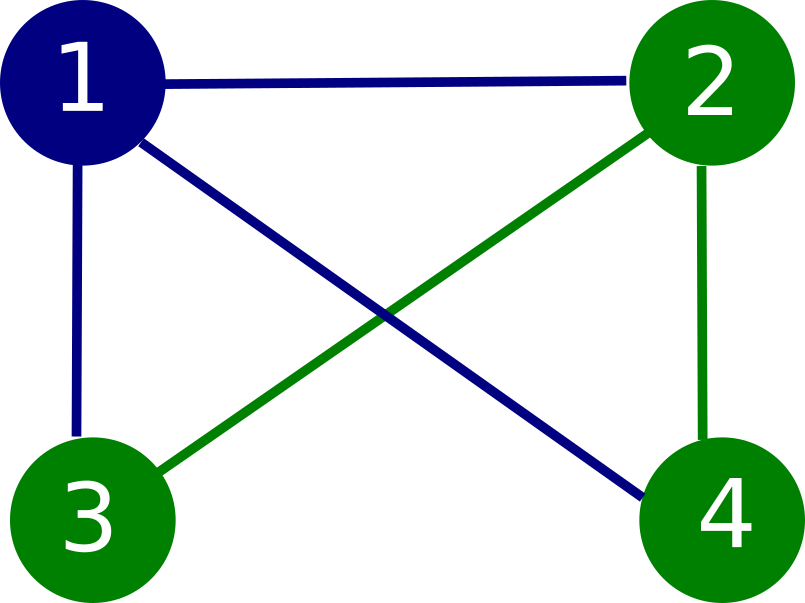
\includegraphics[width=.5\textwidth]{imagens/grafo}
		\end{center}
		
	}
	
	\item (1,5 pt) Qual é o grau do nó 1? E do nó 3?  
	
	\vspace*{0.3cm}
	
	{ \color{blue} {\bf Resposta:} O nó 1 tem grau 3 e o nó 3 tem grau 2.}
	\item (1,5 pt) Indique um caminho do nó 3 ao nó 4 sobre seu desenho de G.
	
	\vspace*{0.3cm}
	
	{ \color{blue} {\bf Resposta:} Indicado de cor {\color{green} \bf verde} na resposta da letra (a).}
\end{enumerate}

\end{enumerate}

\end{document}